%%%%%%%%%%%%%%%%%%%%%%%%%%%%%%%%%%%%%%%%%%%%%%%%%%%%%%%%%
%%             东南大学数电实验报告 LaTeX 模板
%%                SEU-Circuit-Report.cls
%% https://github.com/Teddy-van-Jerry/SEU_Digital_Report
%% ======================================================
%% 版本信息:
%% v1.0 (Nov. 07, 2021)
%% ------------------------------------------------------
%% 模板制作:
%% Teddy van Jerry, (me@teddy-van-jerry.org)
%% * GitHub: https://github.com/Teddy-van-Jerry
%% * Website: https://teddy-van-jerry.org
%% * Blog: https://blog.teddy-van-jerry.org
%% ------------------------------------------------------
%% 使用说明:
%% 1. 编译使用 XeLaTeX 和 Biber
%% 2. 报告基本信息通过修改导言区以 exp 开头的命令
%% 3. 参考文献位于 ref/ref.bib
%% 4. 报告模板依据 MIT License 开源共享
%% ------------------------------------------------------
%% Copyright 2021 (c) Teddy van Jerry
%%
%% Permission is hereby granted, free of charge, to any
%% person obtaining a copy of this software and
%% associated documentation files (the "Software"), to
%% deal in the Software without restriction, including
%% without limitation the rights to use, copy, modify,
%% merge, publish, distribute, sublicense, and/or sell
%% copies of the Software, and to permit persons to whom
%% the Software is furnished to do so, subject to the
%% following conditions:
%%
%% The above copyright notice and this permission notice
%% shall be included in all copies or substantial
%% portions of the Software.
%% 
%% THE SOFTWARE IS PROVIDED "AS IS", WITHOUT WARRANTY OF
%% ANY KIND, EXPRESS OR IMPLIED, INCLUDING BUT NOT
%% LIMITED TO THE WARRANTIES OF MERCHANTABILITY, FITNESS
%% FOR A PARTICULAR PURPOSE AND NONINFRINGEMENT. IN NO
%% EVENT SHALL THE AUTHORS OR COPYRIGHT HOLDERS BE LIABLE
%% FOR ANY CLAIM, DAMAGES OR OTHER LIABILITY, WHETHER IN
%% AN ACTION OF CONTRACT, TORT OR OTHERWISE, ARISING
%% FROM, OUT OF OR IN CONNECTION WITH THE SOFTWARE OR THE
%% USE OR OTHER DEALINGS IN THE SOFTWARE.
%%%%%%%%%%%%%%%%%%%%%%%%%%%%%%%%%%%%%%%%%%%%%%%%%%%%%%%%%%

%% 使用实验报告模板类(字体大小 11pt 约为五号字)
\documentclass[11pt]{SEU-Digital-Report}

%%%%%%%%%%%%%%%%%%%% 报告基本信息 %%%%%%%%%%%%%%%%%%%%
\expno{九} % 实验序号
\expname{时钟实验} % 实验名称
\expauthor{薛宇飞} % 姓名
\expID{04020235} % 学号
\expmates{} % 同组
\expmatesID{} % 学号(同组)
\expmajor{信息工程} % 专业
\explab{金智楼硬件实验室} % 实验室
\expdate{\today} % 实验日期
\expreportdate{\today} % 实验日期
\expgrade{} % 成绩评定
\exptutor{裴文江} % 评阅教师
%%%%%%%%%%%%%%%%%%%%%%%%%%%%%%%%%%%%%%%%%%%%%%%%%%%%
% \usepackage{xeCJK}
\usepackage{threeparttable} %table添加注释
\usepackage{colortbl}
\newcommand{\grayrow}{\rowcolor[rgb]{ .906, .902, .902}}
\usepackage{xcolor}  % tikz画图
\usepackage{tikz}  
\usetikzlibrary{arrows,shapes,chains} 
\usepackage{pgfplots}
\pgfplotsset{compat=1.11}

%% 报告正文
\begin{document}

% 打印封面页
\exptitlepage

\tableofcontents
\newpage

\section{实验目的与内容}       
\begin{enumerate}
    \item 结合实验教材\cite{book,guide},熟悉系统功能调用INT 21H的有关功能。
    \item 编写时钟程序。
\end{enumerate}

\section{\textcolor{red}{预习报告}}
\subsection{实验任务}       
\begin{enumerate}
    \item 执行时钟程序时,屏幕上显示提示符“:” ,由键盘输入当前时、分和秒值,即\texttt{XX:XX:XX√},随即显示时间并不停地计时。
    \item 当有键按下时,立即停止计时,返回\texttt{DOS}。
\end{enumerate}

\subsection{实验原理}
首先利用系统调用INT 21H中02H功能,在CRT上显示一个提示符“:”,要求用户从键盘输入时钟初值(即当前时间),其输入格式为\texttt{XX}(时):\texttt{XX}(分):\texttt{XX}(秒)\texttt{√}。然后利用\texttt{0AH}功能调用接收从键盘输入的字符串,并将接收的字符串存入到缓冲区。

在利用\texttt{0AH}功能调用前要设置一个缓冲区,在调用时,用\texttt{DX}作为输入缓冲区的指针,由键盘输入的字符存入该缓冲区,直至遇到回车键为止。
程序中把输入的‘时’、‘分’、‘秒’初值分别从输入缓冲区中取出,各自放在一个寄存器中,然后调用一个延时1秒钟的子程序,每过1秒使秒值增1,然后检查是否已为60秒,若不是则转显示;若是,则使秒值为0,分值增l,检查是否已为60分,若不是则转显示,若是,则使分值为0,时值增1,接着检查时值是否为24小时,若不是则转显示,若是,则使时值为0,接着也是转显示。
若使程序运行停止,只要有键按下,即可返回\texttt{DOS}。下面列出两种判别是否有键按下的方法:
\begin{enumerate}
    \item 读键扫描码:\\
\begin{lstlisting}[language={[x86masm]Assembler},title=code]
    IN    AL,60H     ;读键扫描码
    TEST  AL, 80H  
    JZ    AAA        ;有键按下,就转AAA
          :
          :
    AAA:  MOV AH,4CH
    INT   21H  
\end{lstlisting}
    \item 调用\texttt{INT 21H}中\texttt{06}功能:\\
\begin{lstlisting}[language={[x86masm]Assembler},title=code]
    MOV   AH,06
    MOV   DL,0FFH        ;判断是否有键按下,有键按下则转AAA
    INT   21H   
    JNZ   AAA
          :
          :
    AAA:  MOV AH,4CH
    INT   21H
\end{lstlisting}
\end{enumerate}

\subsection{流程框图}
实验流程图如图 \ref{fig:process}所示。
\begin{figure}[htbp]
    \centering
    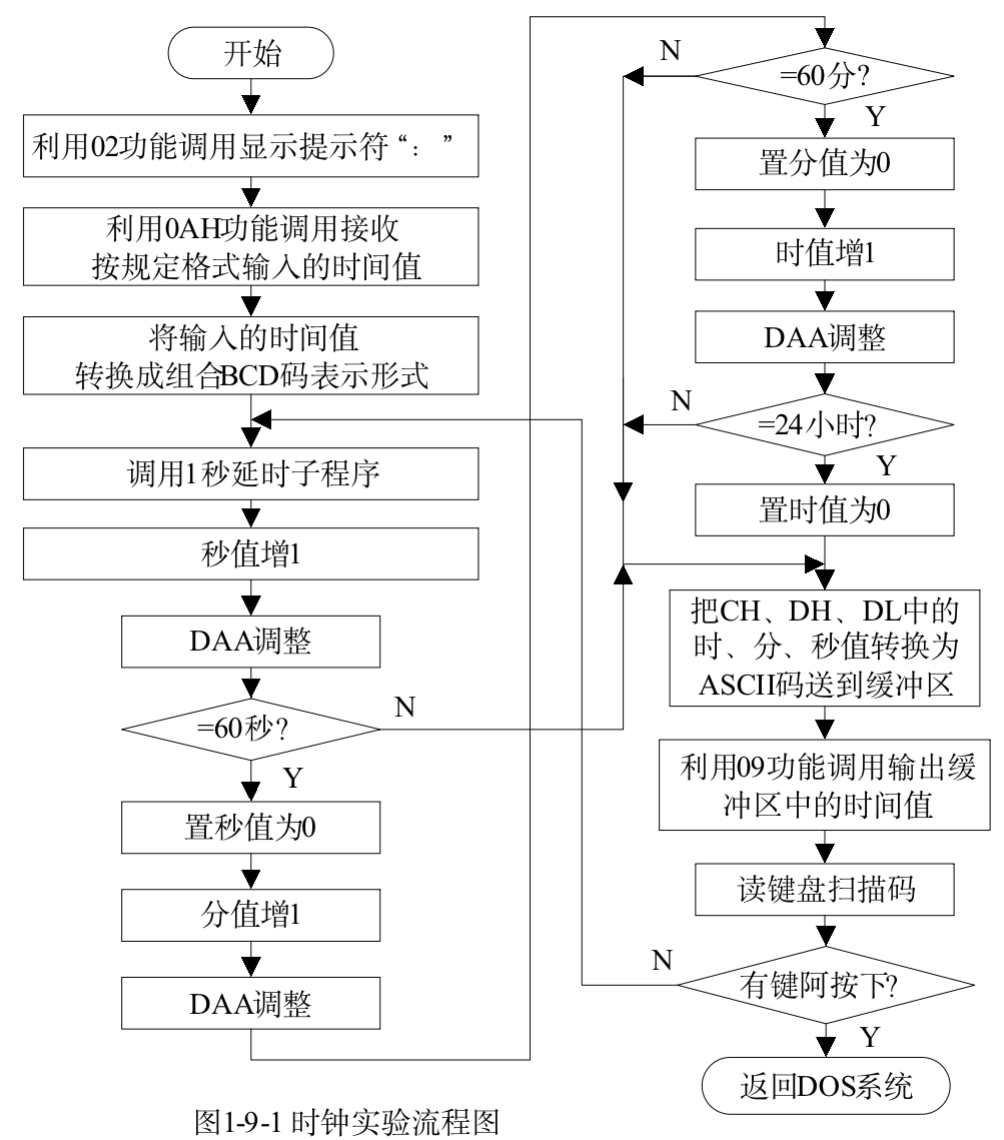
\includegraphics[width=0.7\textwidth]{fig/process.png}
    \caption{}
    \label{fig:process}
\end{figure}

\subsection{实验可能用到的代码}
延时1秒子程序\texttt{DELAY}:
\begin{lstlisting}[language={[x86masm]Assembler},title=delay]
          DELAY  PROC
          PUSH   CX
          PUSH   AX
          MOV    CX,0FFFFH
    GOON: DEC    CX
          JNE    GOON
          POP    AX
          POP    CX
          RET
          DELAY  ENDP
\end{lstlisting}

\section{思考题}
\begin{table}[htbp]
    \centering
    \caption{思考 \label{tab:parameters}}
    \bgroup\def\arraystretch{1.5}
    \setlength{\tabcolsep}{4.5mm}
        \begin{tabular}{l}
          \toprule
          \textbf{实验思考题} \\
          \midrule\midrule
          \grayrow 时钟程序中存在时间误差吗?若有误差,其来源在何处?如何进行误差校正?\\
           bulabula   \\
          \bottomrule
        \end{tabular}
    \egroup
\end{table}

\section{实验调试过程}


\section{附加任务}
\subsection{附加任务1}
在同一行的相同位置显示更新的计时时间,不换行。

\subsection{附加任务2}
输入时间初值时,会检查是否有错、提示错误信息,并可重新输入时间初值。错误提示信息可以分两种:
\begin{enumerate}
    \item 输入的时间初值是错误的字符,即不是数字和冒号;
    \item 输入的时间值是错误的,即“时”大于等于24,“分”和“秒”大于等于60。
\end{enumerate}



\subsection{附加任务3}
延时一秒用\texttt{DOS}系统功能调用实现。

\section{实验总结}
实验总结已随文附在“注意”、“思考”、“分析”中。

% 打印参考文献
\addcontentsline{toc}{section}{参考文献}
\printbibliography

\end{document}
